\documentclass[10pt,fleqn,reqno]{article}

\usepackage{amsmath}
\usepackage{amssymb,amsthm,bm}
\usepackage{pdflscape,afterpage}
\usepackage{tikz}
\usepackage{wrapfig}
\usepackage{tikz-cd}
\usepackage{graphicx}
\usepackage{enumerate}
\usepackage{float,caption,subcaption}
\usepackage[margin=1cm]{caption}
\usepackage[nottoc,numbib]{tocbibind}
\usepackage{setspace}
%\usepackage{times}
\usepackage{mathtools}
\usepackage{ar}	% for aspect ratio \AR command
\usepackage[margin=1.5in]{geometry}

\usepackage[colorlinks=true,linkcolor=blue,citecolor=blue]{hyperref}
\usepackage{fancyhdr}
\pagestyle{fancy}
\fancyhead{}
\fancyfoot{}
\fancyhead[CO]{\textsc{\small Aerodynamic Coefficients}}
\fancyfoot[L]{\href{http://mikef.org}{\emph{\small Michael J. Fairchild}}}
\fancyfoot[R]{\emph{\small Princeton University}}

\usepackage{thmtools}
\declaretheoremstyle[bodyfont=\normalfont,qed=$\triangle$]{example-style}
\declaretheoremstyle[headfont=\scshape,bodyfont=\itshape]{theorem-style}
\declaretheoremstyle[headfont=\itshape,qed=$\triangle$]{remark-style}
\declaretheorem[style=theorem-style]{theorem}
\declaretheorem[style=theorem-style,sibling=theorem]{corollary}
\declaretheorem[style=theorem-style,sibling=theorem]{lemma}
\declaretheorem[style=theorem-style,sibling=theorem]{proposition}
\declaretheorem[style=theorem-style,sibling=theorem]{definition}
\declaretheorem[style=example-style,sibling=theorem]{example}
\declaretheorem[style=example-style,sibling=theorem]{exercise}
\declaretheorem[style=remark-style,sibling=theorem]{remark}

\newcommand\ie{i.e.~}
\newcommand\eg{e.g.~}
\newcommand\vs{vs.~}
\newcommand\defn[1]{\emph{#1}}
\newcommand\od[2]{\frac{d#1}{d#2}}
\newcommand\fd[2]{\frac{\delta #1}{\delta #2}}
\newcommand\pd[2]{\frac{\partial #1}{\partial #2}}
\newcommand\pdn[3]{\frac{\partial^{#3}#1}{\partial #2^{#3}}}
\newcommand\norm[1]{||{#1}||}
\newcommand\varnorm[1]{\left|\left|{#1}\right|\right|}
\newcommand\lrangle[1]{\left\langle #1\right\rangle}
\newcommand\defref[1]{\mbox{Definition \ref{#1}}}
\newcommand\lemref[1]{\mbox{Lemma \ref{#1}}}
\newcommand\thmref[1]{\mbox{Theorem \ref{#1}}}
\newcommand\propref[1]{\mbox{Proposition \ref{#1}}}
\newcommand\corref[1]{\mbox{Corollary \ref{#1}}}
\newcommand\exmref[1]{\mbox{Example \ref{#1}}}
\newcommand\figref[1]{\mbox{Figure \ref{#1}}}
\newcommand\chapref[1]{\mbox{Chapter \ref{#1}}}
\newcommand\appref[1]{\mbox{Appendix \ref{#1}}}
\newcommand\hook{\mathrel{\rule[.0ex]{.6em}{.07em}\rule[.0ex]{.07em}{1.5ex}}\,}
\newcommand\ip{{\mathbf i}}
\newcommand\ed{{\mathbf d}}
\newcommand\ced{{\mathbf D}}
\newcommand\ld{\mathcal L}
\newcommand\T[3]{{{#1}^{#2}}_{#3}}
\DeclareMathOperator\Diff{\mathcal D}
\DeclareMathOperator\Diffvol{\Diff_{\rm{vol}}}
\newcommand\Supp{\text{supp}}
\newcommand\Sect{\Gamma}
\newcommand\Vect{\mathfrak X}
\newcommand\Vectdiv{{\Vect}_{\rm{div}}}
\newcommand\Vectdivpar{{\Vect}_{\rm{div}}^{\parallel}}
\newcommand\Funct{C^\infty}
\renewcommand\emptyset{\varnothing}
\DeclareMathOperator\Orb{\mathcal O}
\DeclareMathOperator\Stab{\mathcal S}
\DeclareMathOperator\Ad{Ad}
\DeclareMathOperator\ad{ad}
\DeclareMathOperator\pr{pr}
\DeclareMathOperator\rank{rank}
\DeclareMathOperator\Emb{Emb}
\DeclareMathOperator\hor{hor}
\DeclareMathOperator\Grad{\nabla}
\DeclareMathOperator\Divg{\nabla\cdot}
\DeclareMathOperator\Curl{\nabla\times}
\newcommand\Lapl{\nabla^2}
\DeclareMathOperator\id{id}
\DeclareMathOperator\Img{img}
\DeclareMathOperator\Ker{ker}
\DeclareMathOperator\sgn{sgn}
\DeclareMathOperator\Span{Span}
\DeclareMathOperator\Trace{tr}
\DeclareMathOperator\Nul{Nul}
\DeclareMathOperator\Mat{\mathcal M}
\DeclareMathOperator\Sym{Sym}
\DeclareMathOperator\Skew{Skew}
\DeclareMathOperator\Ver{ver}
\DeclareMathOperator\Hor{hor}
\DeclareMathOperator\Reyn{Re}
\DeclareMathOperator\Real{Re}
\DeclareMathOperator\Imag{Im}
\DeclareMathOperator\Proj{proj}
\DeclareMathOperator\BL{\mathcal B\mathcal L}

%\title{Aerodynamic Forces, Moments, and Coefficients}
%\author{Michael J. Fairchild\\Dept. of Mechanical and Aerospace Engineering\\Princeton University}
%\date{}
\begin{document}
%\maketitle
%\onehalfspacing
\section{Airfoil geometry}
Figure \ref{fig:airfoil} depicts a finite, three-dimensional airfoil, characterized by its two-dimensional \defn{section} (or \defn{profile}) and its \defn{span}.  Cartesian axes are chosen so that $x,y,z$ encode chordwise, vertical, and spanwise positions, respectively.
\begin{figure}[H]
\begin{center}
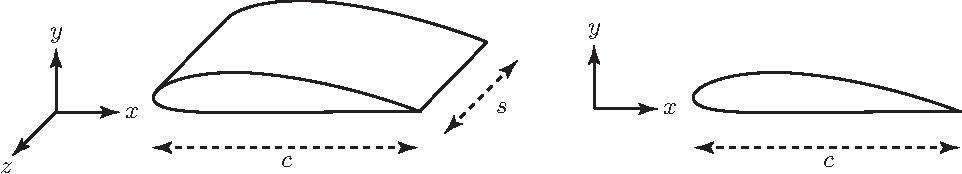
\includegraphics[scale=.8]{Figures/airfoil.pdf}
\caption{Left: a finite, three-dimensional airfoil.  Right: its two-dimensional \defn{section} (or \defn{profile}).  The airfoil \defn{span} and \defn{chord} are denoted $s$ and $c$, respectively.}\label{fig:airfoil}
\end{center}
\end{figure}
The \defn{aspect ratio} $\AR$ of an airfoil is the ratio of the span to the chord, \ie \[\AR:=\frac{\text{span}}{\text{chord}}=\frac{s}{c}.\]  A two-dimensional airfoil should be thought of as the projection onto the $xy$-plane of a three-dimensional airfoil with infinite span; such an airfoil therefore has a formally infinite aspect ratio.

\section{Aerodynamic force, drag, and lift}
The net force and moment on a rigid airfoil are obtained by integrating the pressure and shear stress distributions around its boundary.  We will concentrate on inviscid flows, for which there are no shear stresses, and consequently only the pressure distribution needs to be integrated.  \figref{fig:airfoil-patch} depicts an infinitesimal strip along the surface of an airfoil that is immersed in a uniform background flow $\mathbf u_\infty$.
\begin{figure}[H]
\begin{center}
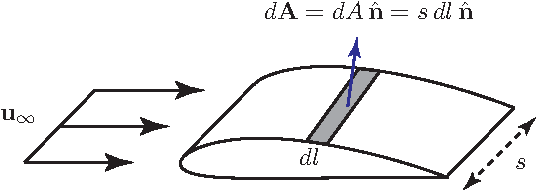
\includegraphics[scale=.8]{Figures/airfoil-patch.pdf}
\caption{Area element $d\mathbf A$ of an infinitesimal strip of an airfoil immersed in a uniform background flow $\mathbf u_\infty$.}\label{fig:airfoil-patch}
\end{center}
\end{figure}
Considering the uniformity of the background flow, symmetry implies that the pressure distribution is constant along the spanwise direction, except possibly at the ends.  As the span increases, the nonuniformity at the ends becomes less important, and in the limit of a two-dimensional airfoil (\ie a spanwise symmetric, three-dimensional airfoil with infinite span), the pressure distribution is exactly independent of spanwise position.  With $\hat{\mathbf n}$ denoting the outward-pointing unit normal vector to the shaded strip, the net force on the strip due to the pressure distribution is \[d\mathbf F = -p\,d\mathbf A = -p\,dA\,\hat{\mathbf n} = -p\,s\,\hat{\mathbf n}\,dl.\]  The net force $\mathbf F_\text{net}$ on the airfoil is obtained by integrating around the airfoil's surface $S$ the forces acting on these patches:
\begin{equation}\label{eqn:net-force}
\mathbf F_\text{net} = \int_S d\mathbf F = -s\oint_C p\,\hat{\mathbf n}\,dl,
\end{equation}
where $C$ is the closed contour describing the airfoil section in the $xy$-plane.  

In numerical simulations, however, we often do not know the pressure itself, but rather the pressure surfeit over the unknown pressure $p_\infty$ at infinity.\footnote{By the \defn{point at infinity} we mean an arbitrary point very far away from the airfoil where the flow is essentially $\mathbf u_\infty$.  We usually take this point to be far upstream of the leading edge.}  That is, although neither $p$ nor $p_\infty$ are known, the difference \mbox{$p-p_\infty$} is known.  Fortunately, this does not present a problem, since the contribution to the net force arising from $p_\infty$ is exactly zero.  Indeed, recall from vector calculus (a proof is given in the appendix) that if $A$ is any region in the plane bounded by a simple closed curve $C$, and if $f:A\to\mathbb R$ is bounded and differentiable on $A$, then \[\oint_{C}f\,\hat{\mathbf n}\,ds = \iint_A\Grad f\,dx\,dy.\]  Since $p_\infty$ is constant, $\Grad p_\infty=0$, and therefore $-s\oint_Cp_\infty\,\hat{\mathbf n}=0$, so this integral may be subtracted from \eqref{eqn:net-force} without changing the result:
\begin{equation}\label{eqn:net-force-infty}
\mathbf F_\text{net} = -s\oint_C(p-p_\infty)\,\hat{\mathbf n}\,dl.
\end{equation}

We now nondimensionalize the force on an airfoil to make it independent of the geometric scale and of the steady background flow.  To do so, define the \defn{dynamic pressure} $q$ as the kinetic energy per unit volume carried by the flow at infinity, \ie \[q:=\frac{1}{2}\rho u_\infty^2,\] where $\rho$ is the density of the fluid (assumed constant).  Meanwhile, the \defn{reference area} $A$ for the airfoil is the product of the span and the chord, \ie \[A:=\text{span}\times\text{chord} = sc = c^2\AR.\]  This is only an approximation to the exact area of the upper surface of the airfoil, but the definition has the advantages of being well defined and being easy to measure for a real airfoil.  The \defn{force coefficient} $C_{\mathbf F}$ is now defined as the dimensionless vector 
\begin{equation}\label{eqn:force-coefficient}
C_{\mathbf F}:=\frac{\mathbf F_\text{net}}{qA}=\frac{\mathbf F_\text{net}}{\frac{1}{2}\rho u_\infty^2sc} = \frac{-1}{c}\oint_C\frac{p-p_\infty}{\frac{1}{2}\rho u_\infty^2}\,\hat{\mathbf n}\,dl.
\end{equation}
Since both $qA$ and $\mathbf F_\text{net}$ carry units of energy per unit length, $C_{\mathbf F}$ is indeed dimensionless.  Note that the span $s$ was eliminated, so this definition is valid for two-dimensional airfoils as well as three-dimensional ones.  

Referring to \figref{fig:drag-lift}, the \defn{drag force} $\mathbf F_D$ and \defn{lift force} $\mathbf F_L$ are the components of the net aerodynamic force parallel and perpendicular to, respectively, the onset flow $\mathbf u_\infty$.
\begin{figure}[H]
\begin{center}
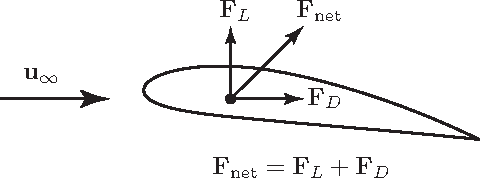
\includegraphics[scale=.8]{Figures/drag-lift.pdf}
\caption{The drag and lift forces on an airfoil are the components of the net aerodynamic force parallel and perpendicular to, respectively, the onset flow.}\label{fig:drag-lift}
\end{center}
\end{figure}
If $\hat{\mathbf d}:=\frac{\mathbf u_\infty}{\norm{\mathbf u_\infty}}$ is the unit vector in the drag direction, and if $\hat{\mathbf l}$ is the unit vector in the lift direction, the magnitudes of the drag and lift forces are \[F_D:=\mathbf F_\text{net}\cdot\hat{\mathbf d},\quad F_L:=\mathbf F_\text{net}\cdot\hat{\mathbf l}.\]  As with the net aerodynamic force, it is useful to define the nondimensional \defn{drag coefficient} $C_D$ and \defn{lift coefficient} $C_L$ by normalizing the respective force magnitudes by the dynamic pressure and the reference area:
\begin{align*}
C_D:&=\frac{F_D}{qA}=\frac{\mathbf F_\text{net}\cdot\hat{\mathbf d}}{qA} = C_{\mathbf F}\cdot\hat{\mathbf d},\\
C_L:&=\frac{F_L}{qA}=\frac{\mathbf F_\text{net}\cdot\hat{\mathbf l}}{qA} = C_{\mathbf F}\cdot\hat{\mathbf l}.
\end{align*}

\section{Pressure coefficient}
The equation for the force coefficient, \eqref{eqn:force-coefficient}, suggests that we define the \defn{pressure coefficient} $C_p$ as the dimensionless ratio \[C_p:=\frac{p-p_\infty}{\frac{1}{2}\rho u_\infty^2}.\]  Then the force coefficient is simply \[C_{\mathbf F}=\frac{-1}{c}\oint_C C_p\,\hat{\mathbf n}\,dl.\]  The working assumption so far has been that the fluid is inviscid.  To compute the pressure distribution, we now make the additional assumption that the fluid is incompressible.  If $D$ is a simply connected region on which the flow is \defn{irrotational} (\ie $\Curl\mathbf u = 0$), it is a theorem that there exists a \defn{vector potential} $\phi:D\to\mathbb R$ such that $\mathbf u=\Grad\phi$.  For this reason, irrotational flow of an inviscid incompressible fluid in a simply connected region is called \defn{potential flow}.  The Bernoulli equation, expressing conservation of energy, is \[\pd{\phi}{t}+\frac{u^2}{2}+\frac{p}{\rho} = C(t),\] where $C(t)$ is a constant throughout $D$ but may well depend on time.  Assuming we take the point at infinity as lying in the region $D$, then Bernoulli's equation implies that \[\pd{\phi}{t}+\frac{u^2}{2}+\frac{p}{\rho} = \pd{\phi_\infty}{t}+\frac{u_\infty^2}{2}+\frac{p_\infty}{\rho},\] where the quantities on the left are computed at an arbitrary point $\mathbf x\in D$, and the quantities on the right are computed at the point at infinity.  The preceding display rearranges to \[C_p=\frac{p-p_\infty}{\frac{1}{2}\rho u_\infty^2} = 1-\frac{u^2}{u_\infty^2}-\frac{2}{u_\infty^2}\pd{}{t}(\phi-\phi_\infty).\]  For steady flow, the potential is constant in time, so that $\pd{}{t}(\phi-\phi_\infty)=0$, and the pressure coefficient simplifies to the well-known formula $C_p=1-(\frac{u}{u_\infty})^2$.  For unsteady flows, the potential term does not vanish.  To compute the potential at the point $\mathbf x\in D$, we use the fact that $\mathbf u=\nabla\phi$ implies $\phi(\mathbf x) = \phi_\infty + \int_\infty^{\mathbf x}\Grad\phi\cdot d\mathbf s$, where the lower limit of integration signifies the point at infinity.  Since $\Grad\phi = \mathbf u$, this may be rearranged to \[\phi(\mathbf x)-\phi_\infty = \int_\infty^{\mathbf x}\mathbf u\cdot d\mathbf s.\]  Hence the preceding expression for $C_p$ can be written \[C_p(\mathbf x) = 1-\frac{u^2(\mathbf x)}{u_\infty^2}-\frac{2}{u_\infty^2}\pd{}{t}\int_\infty^{\mathbf x}\mathbf u\cdot d\mathbf s,\quad \text{for~}\mathbf x\in D.\]  Assuming the flow field is known everywhere, as it typically is during a numerical computation, the integral term may be computed by selecting a fixed point far upstream of the airfoil to be considered as the point at infinity.

\section{Aerodynamic moment; center of pressure}
Now that forces have been computed, we turn our attention to rotational moments.  For an airfoil, the most important consideration is that of pitch rotations about a spanwise axis, as shown in \figref{fig:moment}.
\begin{figure}[H]
\begin{center}
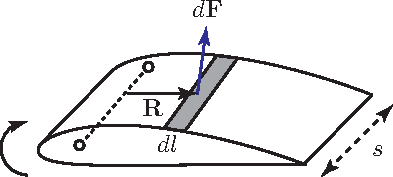
\includegraphics[scale=.8]{Figures/moment.pdf}
\caption{Pitch rotations about a spanwise axis}\label{fig:moment}
\end{center}
\end{figure}
Let $\mathbf R$ be the displacement vector from the pitch axis to a patch on the surface $S$ of the airfoil.  Since the pitch axis is take spanwise, the vector $\mathbf R$ is constant along infinitesimal spanwise surface strips, and the net moment $d\mathbf M$ on the strip due to the pressure distribution is \[d\mathbf M = \mathbf R\times d\mathbf F=-s\,p\,\mathbf R\times\hat{\mathbf n}\,dl.\]  Integrating over the airfoil surface $S$ the moments on each patch gives the net moment $\mathbf M$ on the airfoil as \[\mathbf M:=\int_Sd\mathbf M=-s\oint_C p\,\mathbf R\times\hat{\mathbf n}\,dl.\]  As before, we often know $p-p_\infty$ rather than $p$ or $p_\infty$.  It is proved in the appendix that $\oint_C\mathbf R\times\hat{\mathbf n}\,dl=0$.  Since $p_\infty$ is constant over the airofil surface, $-s\oint_Cp_\infty\,\mathbf R\times\hat{\mathbf n}\,dl=-s\,p_\infty\oint_C\,\mathbf R\times\hat{\mathbf n}\,dl=0$.  Hence this may be subtracted from the equation for $\mathbf M$ without altering the result, giving \[\mathbf M=-s\oint_C(p-p_\infty)\,\mathbf R\times\hat{\mathbf n}\,dl.\]  To nondimensionalize the moment, which is a distance times a force, we normalize the force factor in the same manner as $\mathbf F_\text{net}$ was normalized to $C_{\mathbf F}$, \ie by the product of the dynamic pressure $q=\frac{1}{2}\rho u_\infty^2$ and the reference area $A=sc$, but we must also normalize the distance factor, with the natural choice being to normalize it by the chord length $c$.  Hence if $\mathbf M$ is the moment about a specified axis, we define the \defn{moment coefficient} $C_{\mathbf M}$ by \[C_{\mathbf M}:=\frac{\mathbf M}{qAc}=\frac{1}{sc^2}\left(-s\oint_C\frac{p-p_\infty}{\frac{1}{2}\rho u_\infty^2}\,\mathbf R\times\hat{\mathbf n}\,dl\right)=\frac{-1}{c^2}\oint_CC_p\,\mathbf R\times\hat{\mathbf n}\,dl.\]

As defined in this section, a positive moment induces a counterclockwise rotation of a two-dimensional airfoil.  It is customary in aerodynamics, however, to arrange the definition so that a positive moment induces a pitch-up motion, and so care must be used in choosing the correct sign of $C_{\textbf M}$ based on the convention in effect.

We now show that it is only necessary to compute the pitching moment about a single axis, and that all other moments may be computed from this.  It is natural to choose the airfoil's leading edge, about which $\mathbf R_\text{LE}$ denotes the displacement vector from this axis to a surface patch, and $\mathbf M_\text{LE}$ denotes the resulting moment.  Consider another spanwise axis, displaced from the leading edge by $\mathbf R_0$.  If $\mathbf R$ is the displacement vector from this new axis to an airfoil patch, then $\mathbf R_\text{LE}=\mathbf R_0+\mathbf R$ is the displacement from the leading edge axis to the given patch. Hence the moment $\mathbf M$ about this axis is
\begin{align*}
\mathbf M &= -s\oint_C(p-p_\infty)(\mathbf R_\text{LE}-\mathbf R_0)\times\hat{\mathbf n}\,dl\\
&=-s\oint_C(p-p_\infty)\mathbf R_\text{LE}\times\hat{\mathbf n}\,dl-\mathbf R_0\times\left(-s\oint_C(p-p_\infty)\,\hat{\mathbf n}\,dl\right).
\end{align*}
The first integral equals $\mathbf M_\text{LE}$, and the second integral equals $\mathbf F_\text{net}$, so \[\mathbf M=\mathbf M_\text{LE}-\mathbf R_0\times\mathbf F_\text{net},\] or in nondimensional form, \[C_{\textbf M} = \frac{\mathbf M}{qAc} = C_{\textbf M,LE}-\frac{\mathbf R_0}{c}\times C_{\mathbf F}.\]

Now that forces and moments have been defined, we can introduce an additional concept from aerodynamics.  When the net aerodynamic force is nonzero, the \defn{center of pressure} is the point at which the force acts to produce the observed moment about the pitch axis.  When defined, the center of pressure lies along the pitch axis if and only if the moment about this axis is zero.  It is possible for the center of pressure to lie outside the airfoil, although this is somewhat unusual.  For thin symmetric airfoils, it is well known that the center of pressure for pitching about the leading edge is approximately the quarter-chord point.

%Meanwhile, the \defn{aerodynamic center} TODO.  This is much harder to compute.

\section{Power, thrust, and efficiency}
Consider forward motion of the airfoil through the fluid, \ie motion that is directed, on average, opposite to the onset flow $\mathbf u_\infty$.  The airfoil's position is described by coordinates $(x,y)$ of a fixed point on the airfoil (say, its leading edge), together with its pitch angle $\theta$ about the pitch axis.  Throughout its motion, the airfoil is subject to a time-varying net force $\mathbf F(t)=F_x(t)\,\hat{\mathbf x}+F_y(t)\,\hat{\mathbf y}$ and a time-varying moment $\mathbf M(t)=M(t)\,\hat{\mathbf z}$.  If $T$ denotes the period of one cycle of the motion, we let $P_\text{out}$, $P_\text{in}$, and $\eta$ denote the output power, input power, and propulsive efficiency during during a period of one cycle, \ie
\begin{align*}
P_\text{out} &:= \frac{1}{T}\int_0^T F_xu_\infty\,dt,\\
P_\text{in} &:= \frac{1}{T}\int_0^T F_y\od{y}{t}\,dt+\frac{1}{T}\int_0^TM\od{\theta}{t}\,dt,\\
\eta &:= \frac{P_\text{out}}{P_\text{in}}.
\end{align*}
The \defn{power coefficient} $C_P$ is the nondimensionalized average power input over one cycle, \[C_P:=\frac{P}{(\frac{1}{2}\rho u_\infty^2)(Au_\infty)},\] where $A=sc$ is the reference area of the airfoil.  The \defn{thrust coefficient} $C_T$ is the nondimensionalized average thrust force over one cycle, \[C_T:=\frac{F}{(\frac{1}{2}\rho u_\infty^2)A}.\]  The \defn{propulsive efficiency} $\eta$ is the ratio of the thrust coefficient (output) to the power coefficient (input), \[\eta:=\frac{C_T}{C_P}=\frac{Fu_\infty}{P}.\]

\begin{appendix}
\section{Proofs}
\begin{theorem} If $A$ is a region bounded by a simple closed curve $C$ in the plane with outward-pointing normal $\hat{\mathbf n}$, and if $f:A\to\mathbb R$ is bounded and differentiable, then \[\oint_C f\,\hat{\mathbf n}\,dl = \iint_A\Grad f\,dx\,dy.\]
\end{theorem}
\begin{proof} This may be proved with Gauss' theorem.  Working in Cartesian $x,y$ coordinates, write $\hat{\mathbf n}=(n_x,n_y)$ and $\Grad f=(\pd{f}{x},\pd{f}{y})$.  Then \[\iint_A\Grad f\,dx\,dy = \left(\iint_A\pd{f}{x}\,dx\,dy,\iint_A\pd{f}{y}\,dx\,dy\right).\]  Noting that $\pd{f}{x} = \Divg(f,0)$, Gauss' theorem implies \[\iint_A\pd{f}{x}\,dx\,dy = \iint_A\Divg(f,0)\,dx\,dy = \oint_C (f,0)\cdot\hat{\mathbf n}=\oint_C f\,n_x\,dl.\]  Since an analogous result holds for the $y$ component, the result is proved.
\end{proof}
\begin{theorem} If $C$ is any simply closed curve in the plane, if $\mathbf r$ denotes the position vector to points along $C$, and if $\hat{\mathbf n}$ is the outward-pointing unit normal vector along $C$, then \[\oint_C\mathbf r\times\hat{\mathbf n}\,dl = 0.\]
\end{theorem}
\begin{proof} In Cartesian coordinates, let $\mathbf r=(x,y)$ denote points along the curve $C$, and let $\hat{\mathbf n}=(n_x,n_y)$ and $\hat{\mathbf t}=(t_x,t_y)$ denote the unit outward-pointing normal and positively oriented tangent vectors along $C$, respectively.  Then \[\oint_C\mathbf r\times\hat{\mathbf n}\,dl = \hat{\mathbf z}\oint_C x\,n_y-y\,n_x\,dl,\] where $\hat{\mathbf z}$ is the unit normal to the $x,y$ plane.  The components of the normal and tangent vectors are related by $n_x = t_y$ and $n_y=-t_x$, so \[\oint_C\mathbf r\times\hat{\mathbf n}\,dl = \hat{\mathbf z}\oint_C x(-t_x)-y(t_y)\,dl=-\hat{\mathbf z}\oint_C\mathbf r\cdot d\mathbf s,\] where $d\mathbf s=\hat{\mathbf t}\,dl$ is the arc-length-parameterized line element along $C$.  Finally, since $\mathbf r = \frac{1}{2}\nabla(x^2+y^2)$, the integral vanishes because it is the integral around a closed loop of the gradient of a scalar function.
\end{proof}
\end{appendix}
\end{document}